To lay the foundation for our study of agent failures and debugging, this section introduces two \textit{proposed} components. Section~\ref{sub:aet} presents the \AET{}, a structured framework that organizes recurring failure modes into coherent modules. Section~\ref{sub:bench} then describes the \Bench{}, which grounds this taxonomy in systematically annotated trajectories from multiple environments. 

\begin{figure}[h]
    \centering
    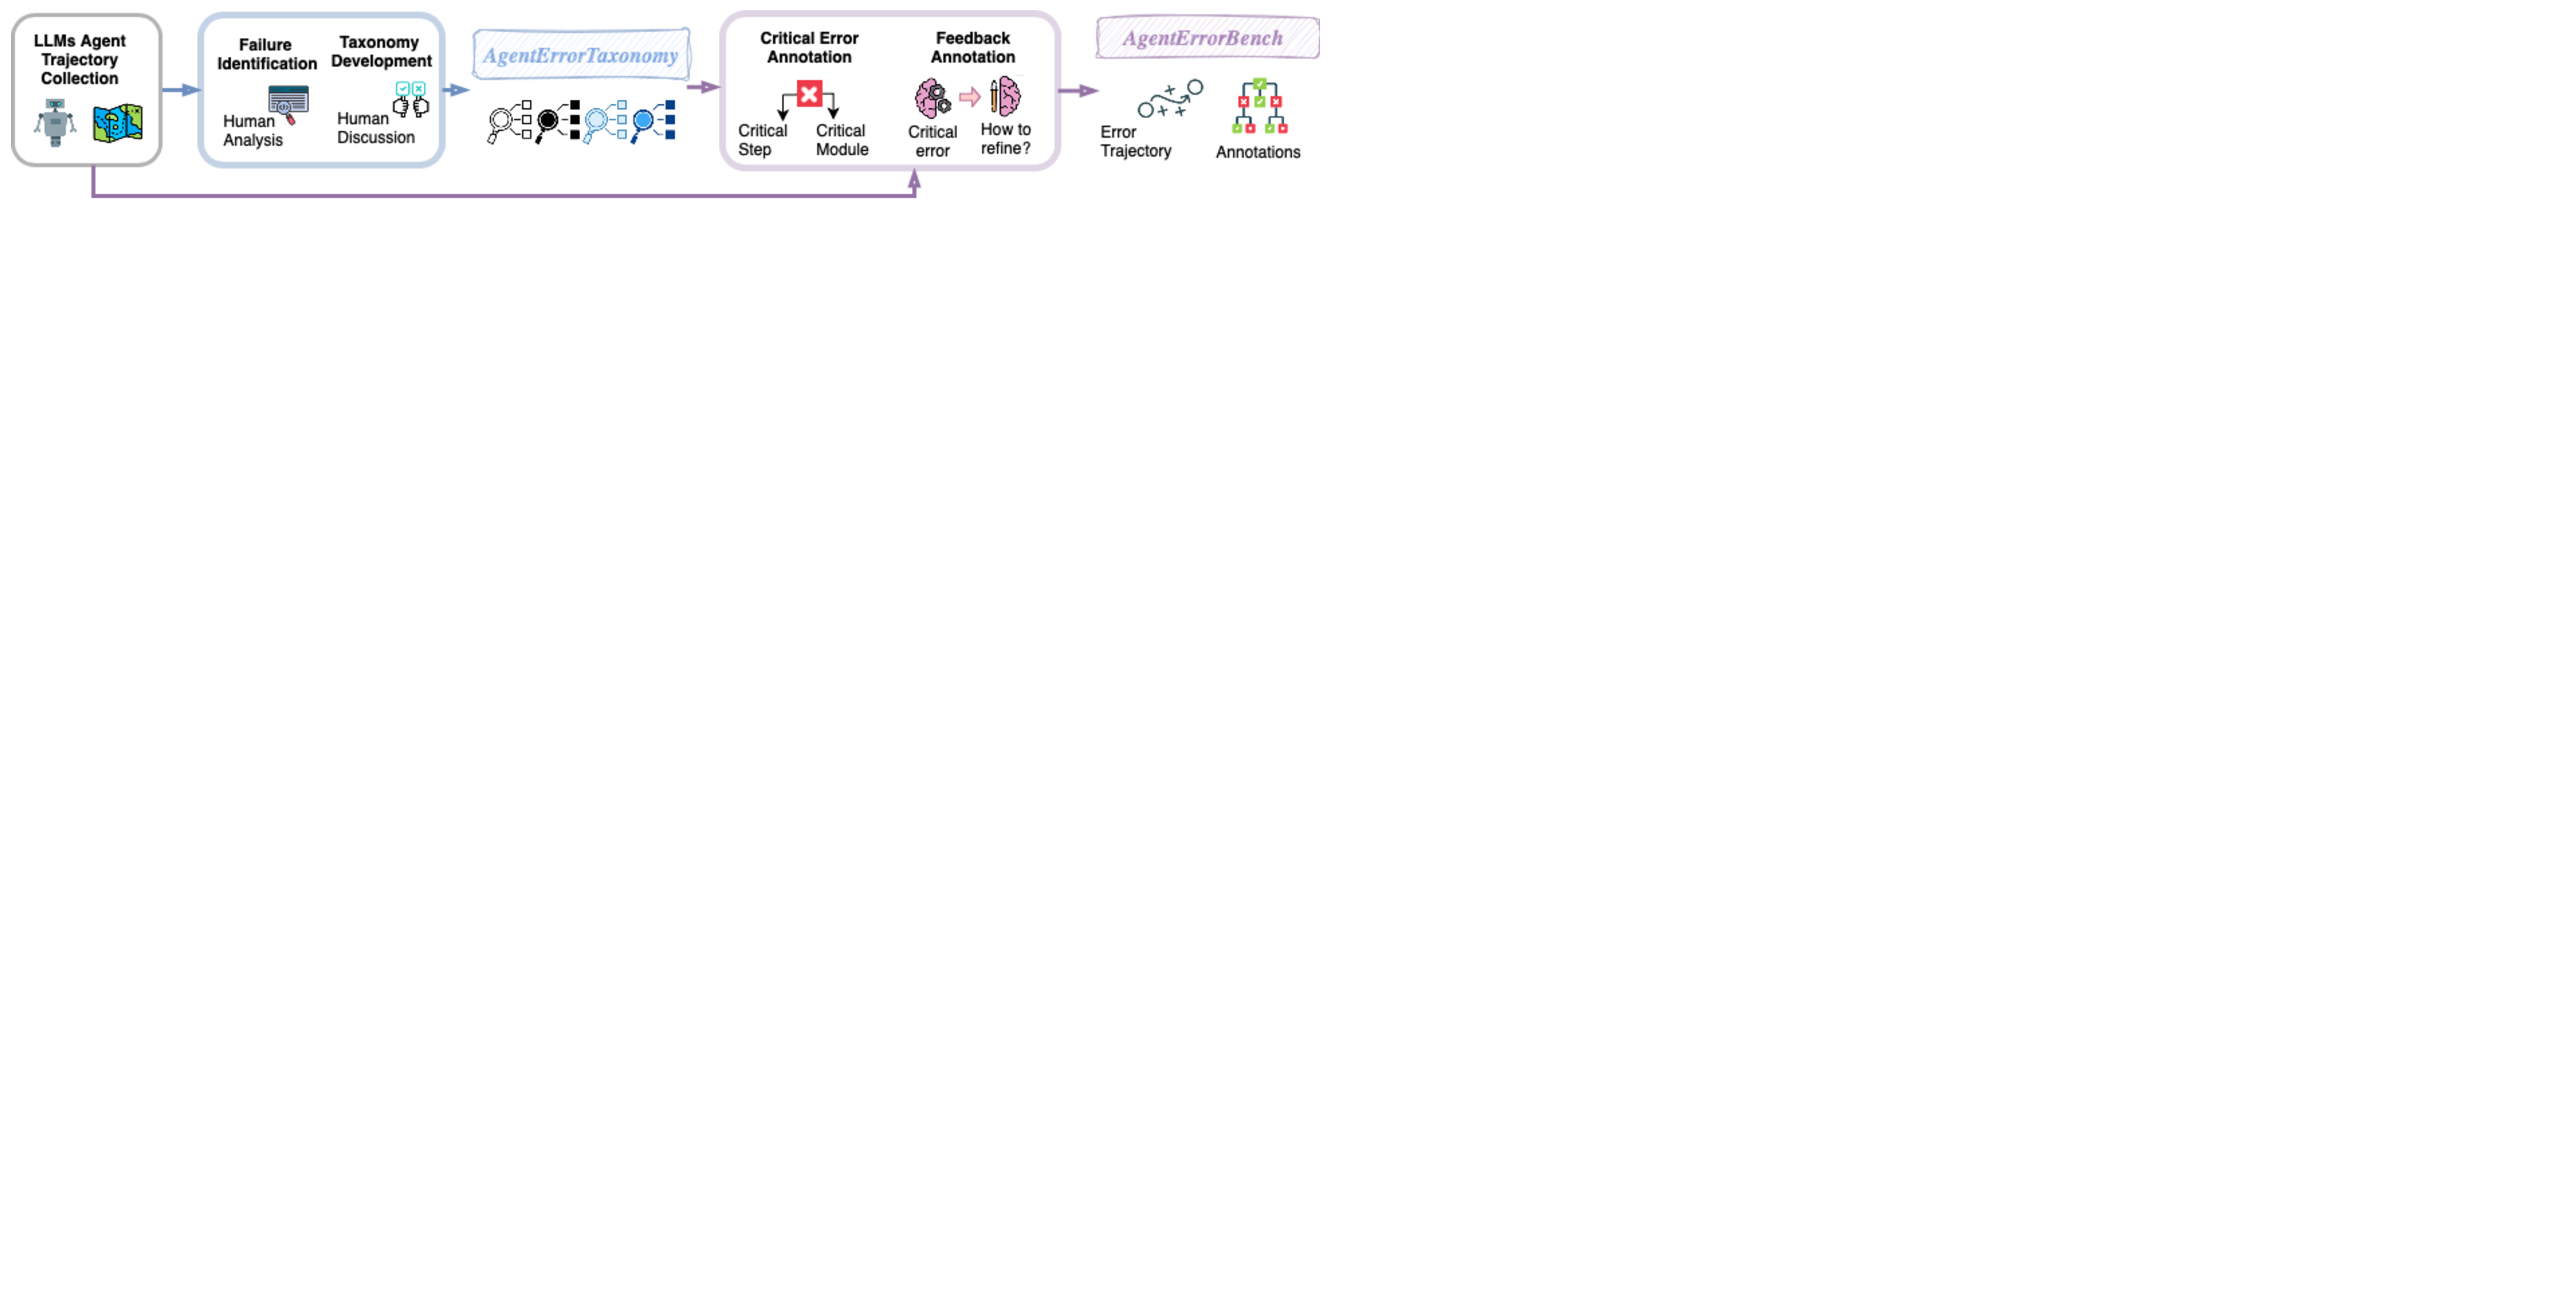
\includegraphics[width=1\linewidth]{iclr2026/figures/aet_bench.pdf}
    \caption{\textbf{Pipeline of proposed \AET{} and \Bench{}}. Failed trajectories are collected, analyzed to develop a taxonomy of errors, and then annotated with root causes and actionable feedback to form the benchmark.}
    \label{fig:aet_bench_construction}
    \vspace{-0.2in}
\end{figure}

\subsection{Agent Failure Analysis}
\label{sub:aet}

To systematically investigate how agents fail, we collected over 500 failed trajectories from ALFWorld, WebShop, and GAIA, and conducted detailed human analyses to uncover recurring patterns. 
This study revealed the following central insight:

\begin{tcolorbox}[colback=berkeleyblue!5!white, colframe=berkeleyblue!100!black, boxrule=0.5mm, left=0.1mm, right=0.1mm, top=0.1mm, bottom=0.1mm]
\textbf{\textit{Key Insight.}} \textit{Error propagation is the primary bottleneck in LLM agent reliability.}  
Early mistakes rarely remain confined; instead, they cascade into subsequent steps, distorting reasoning, compounding misjudgments, and ultimately derailing the entire trajectory.
\end{tcolorbox}

Building on this insight, we introduce the \AET{}, a structured taxonomy that organizes recurring failure modes into five modules. Four capture the core operations of an agent—\textit{memory}, \textit{reflection}, \textit{planning}, and \textit{action}—while a fifth category accounts for \textit{system-level} errors that arise from external tools or infrastructure. This modular view not only enumerates common error types but also clarifies how weaknesses in one stage can cascade into others, enabling a principled approach to tracing and diagnosing failures.

\tcbset{
  colback=white,
  colframe=black!50,
  arc=4pt, % corner radius
  boxrule=0.5pt,
  left=2pt,
  right=2pt,
  top=2pt,
  bottom=2pt
}

\small
\begin{tcolorbox}
\begin{tabular}{>{\bfseries}m{0.18\linewidth} m{0.75\linewidth}}

\rowcolor{orange!10} \textit{Memory} & Errors in recalling or retrieving information (false recall, omission, retrieval failure) that distort subsequent reasoning. \\

\rowcolor{blue!10} \textit{Reflection} & Failures in monitoring progress or interpreting outcomes (progress misassessment, outcome misinterpretation), blocking course correction. \\

\rowcolor{green!10} \textit{Planning} & Logically unsound or infeasible strategies (impossible actions, constraint ignorance, incoherent subgoals) that cascade into missteps. \\

\rowcolor{yellow!15} \textit{Action} & Mistakes in executing operations (malformed outputs, incorrect parameters, missing arguments) that are visible but often mask upstream errors. \\

\rowcolor{red!15} \textit{System-level} & Failures outside reasoning, such as tool crashes, API mismatches, or exceeding step limits, highlighting system robustness issues. \\

\end{tabular}
\end{tcolorbox}

The \AET{} is designed not merely as a catalog of errors but as a causal lens for understanding how failures originate, propagate, and interact across modules. Full definitions are provided in Appendix~\ref{app:aet}.

\subsection{Agent Error Benchmark}
\label{sub:bench}

To rigorously evaluate whether models can detect critical errors and produce actionable feedback, we construct the \Bench{}. This benchmark grounds the taxonomy in real-world trajectories, offering the first standardized testbed for error detection and debugging.

The construction pipeline is shown in Figure~\ref{fig:aet_bench_construction}. We curated 200 representative trajectories: 100 from ALFWorld, 50 from WebShop, and 50 from GAIA. Ten expert annotators—graduate students with prior experience in NLP and LLMs agent research—labeled each trajectory using the \AET{} schema. Annotation proceeded at the decision-step level: every action, reflection, or plan was reviewed, and annotators tagged its error type(s) according to the taxonomy. In addition, they were tasked with identifying the minimal set of root-cause failures that explain the downstream error cascade, rather than exhaustively flagging all surface mistakes. This root-cause focus was emphasized through detailed guidelines and calibration examples, refined iteratively over three rounds of pilot annotation.

To ensure consistency, annotators first completed a training phase with feedback from the authors, followed by independent double-annotation on a shared subset of trajectories. Disagreements were adjudicated collectively, leading to several clarifications in category definitions (e.g., distinguishing “retrieval failure” under memory vs. “constraint ignorance” under planning). The final protocol balanced granularity with reliability, aiming for concise but causally meaningful tags. Inter-annotator agreement, measured using Cohen’s $\kappa$, reached $\kappa = \text{0.55}$ across modules, indicating substantial agreement.

The resulting dataset provides a quantitative view of how agents fail in practice. Figure~\ref{fig:failure_analysis} shows how errors emerge across steps, modules, and error types in the \Bench{}. It shows most failures cluster in mid-trajectory steps (6–15), where early missteps often cascade downstream. Memory and reflection dominate, with retrieval failures, hallucinations, and progress misjudgments leading to flawed planning. Action and system errors occur less frequently but remain critical, as malformed outputs or step-limit exhaustion can immediately terminate trajectories. The complete error type distribution is attached to Appendix \ref{app:failure_analysis}. 


\begin{figure}[htbp]
    \centering
    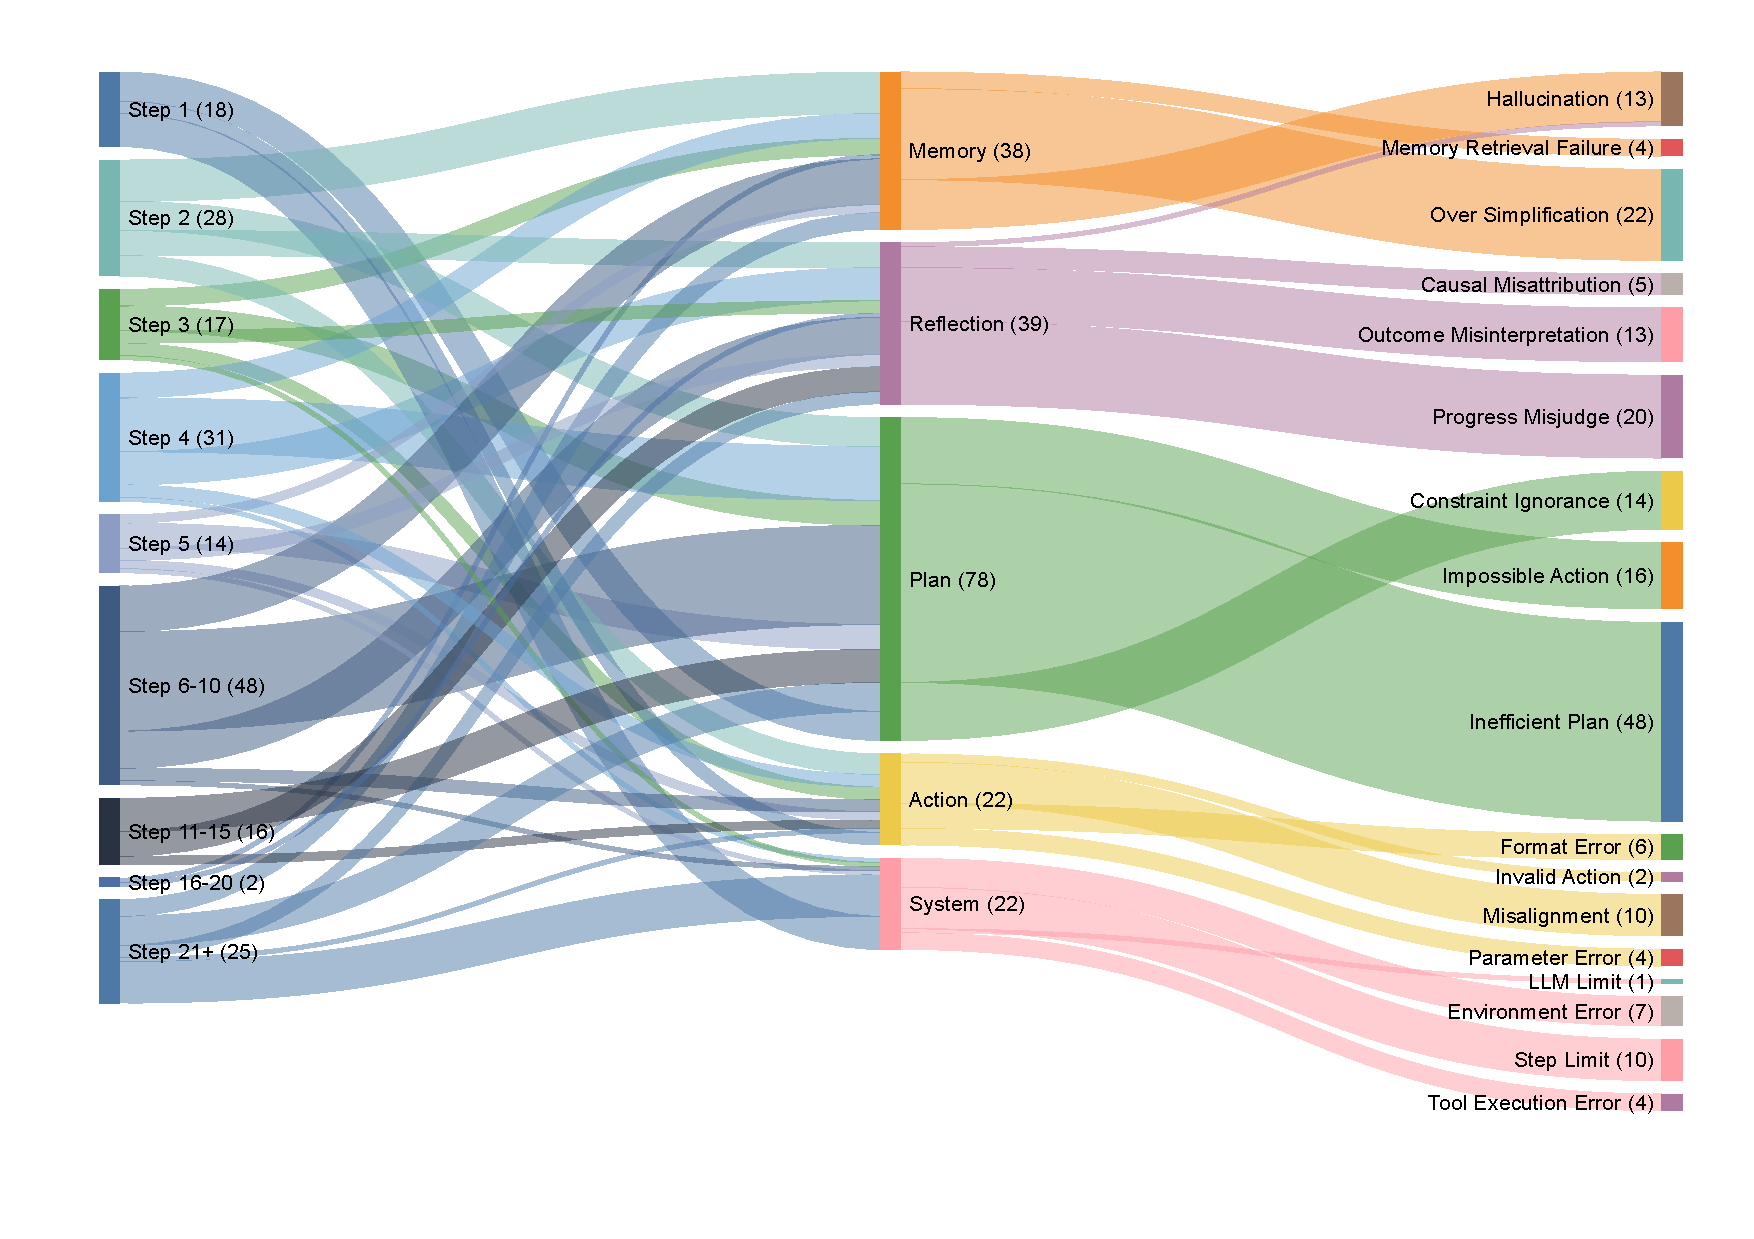
\includegraphics[width=0.96\linewidth]{iclr2026/figures/Combined_Sankey.pdf}
    \caption{Distribution of failure cases in LLM agents on the \Bench{}}
    \label{fig:failure_analysis}
\end{figure}


Together, \AET{} and \Bench{} provide both the conceptual foundation and the empirical infrastructure for advancing robust LLM agents.
